%% Copyright 2022 OXFORD UNIVERSITY PRESS
%%
%% This file is part of the 'oup-authoring-template Bundle'.
%% ---------------------------------------------
%%
%% It may be distributed under the conditions of the LaTeX Project Public
%% License, either version 1.2 of this license or (at your option) any
%% later version.  The latest version of this license is in
%%    http://www.latex-project.org/lppl.txt
%% and version 1.2 or later is part of all distributions of LaTeX
%% version 1999/12/01 or later.
%%
%% The list of all files belonging to the 'oup-authoring-template Bundle' is
%% given in the file `manifest.txt'.
%%
%% Template article for OXFORD UNIVERSITY PRESS's document class `oup-authoring-template'
%% with bibliographic references
%%

%%%CONTEMPORARY%%%
% \documentclass[unnumsec,webpdf,contemporary,large]{oup-authoring-template}%
\documentclass[unnumsec,webpdf,contemporary,large,namedate]{oup-authoring-template}% uncomment this line for author year citations and comment the above
%\documentclass[unnumsec,webpdf,contemporary,medium]{oup-authoring-template}
%\documentclass[unnumsec,webpdf,contemporary,small]{oup-authoring-template}

%%%MODERN%%%
%\documentclass[unnumsec,webpdf,modern,large]{oup-authoring-template}
% \documentclass[unnumsec,webpdf,modern,large,namedate]{oup-authoring-template}% uncomment this line for author year citations and comment the above
%\documentclass[unnumsec,webpdf,modern,medium]{oup-authoring-template}
%\documentclass[unnumsec,webpdf,modern,small]{oup-authoring-template}

%%%TRADITIONAL%%%
%\documentclass[unnumsec,webpdf,traditional,large]{oup-authoring-template}
% \documentclass[unnumsec,webpdf,traditional,large,namedate]{oup-authoring-template}% uncomment this line for author year citations and comment the above
%\documentclass[unnumsec,namedate,webpdf,traditional,medium]{oup-authoring-template}
%\documentclass[namedate,webpdf,traditional,small]{oup-authoring-template}

%\onecolumn % for one column layouts

%\usepackage{showframe}

\graphicspath{{Fig/}}

% line numbers
% \usepackage[mathlines, switch]{lineno}
% \usepackage[right]{lineno}

\theoremstyle{thmstyleone}%
\newtheorem{theorem}{Theorem}%  meant for continuous numbers
%%\newtheorem{theorem}{Theorem}[section]% meant for sectionwise numbers
%% optional argument [theorem] produces theorem numbering sequence instead of independent numbers for Proposition
\newtheorem{proposition}[theorem]{Proposition}%
%%\newtheorem{proposition}{Proposition}% to get separate numbers for theorem and proposition etc.
\theoremstyle{thmstyletwo}%
\newtheorem{example}{Example}%
\newtheorem{remark}{Remark}%
\theoremstyle{thmstylethree}%
\newtheorem{definition}{Definition}

%% add custom package
\usepackage[detect-all=true]{siunitx}
\DeclareSIUnit\molar{\mole\per\cubic\deci\metre}
\DeclareSIUnit\Molar{\textsc{m}}
\DeclareSIUnit\gee{\textit{g}}
\DeclareSIUnit\Units{\textnormal{U}}
\DeclareSIUnit\rpm{\textnormal{rpm}}
\DeclareSIUnit\pixel{\textnormal{px}}
\DeclareSIUnit\electron{\textnormal{e\textsuperscript{--}}}
\sisetup{
	round-mode = places,
	round-precision = 2
}%

\usepackage{booktabs}
\usepackage{minted}
\usepackage[acronym, style=index, shortcuts]{glossaries-extra}
\usepackage{cleveref}
\usepackage{adjustbox}
\usepackage{xr}
\externaldocument{supplementary_information}

% define new commands
\newcommand\pcref[1]{(\cref{#1})}
\newcommand\pCref[1]{(\Cref{#1})}

%\makeglossaries

\newacronym{blat}{BLAT}{BLAST-like alignment tool}
\newacronym{blast}{BLAST}{Basic Local Alignment Search Tool}

\newacronym{cli}{CLI}{command-line interface}
\newacronym{api}{API}{application programming interface}
\newacronym{ide}{IDE}{Integrated Development Environment}
\newacronym{gil}{GIL}{Global Interpreter Lock}
\newacronym{ci}{CI}{continuous integration}
\newacronym{cd}{CD}{continuous development}
\newacronym{ucsc}{UCSC}{UCSC Genome Browser}
\newacronym{hsp}{HSP}{high-scoring pair}
\newglossaryentry{pxblat}{name=PxBLAT, description={pxblat}}
% define new commands


\begin{document}

\journaltitle{Journal Title Here}
\DOI{DOI HERE}
\copyrightyear{2024}
\pubyear{2024}
\access{Advance Access Publication Date: Day Month Year}
\appnotes{Paper}

\firstpage{1}

%\subtitle{Subject Section}

\title[Efficient Genomics Analysis with \gls{pxblat}]{PxBLAT: An Efficient Python Binding Library for BLAT}

\author[1]{Yangyang Li\ORCID{0000-0001-8224-1067}}
% \author[2]{Second Author}
% \author[3]{Third Author}
% \author[3]{Fourth Author}
\author[1,2,$\ast$]{Rendong Yang\ORCID{0000-0002-9512-2240}}

\authormark{Li and Yang}

\address[1]{\orgdiv{Department of Urology}, \orgname{Northwestern University, Feinberg School of Medicine}, \orgaddress{\street{Chicago}, \state{IL}, \postcode{60611}, \country{USA}}}
\address[2]{\orgdiv{Robert H. Lurie Comprehensive Cancer Center}, \orgname{Northwestern University Feinberg School of Medicine}, \orgaddress{\street{Chicago}, \state{IL}, \postcode{60611}, \country{USA}}}
% \address[3]{\orgdiv{Department}, \orgname{Organization}, \orgaddress{\street{Street}, \postcode{Postcode}, \state{State}, \country{Country}}}
% \address[4]{\orgdiv{Department}, \orgname{Organization}, \orgaddress{\street{Street}, \postcode{Postcode}, \state{State}, \country{Country}}}

\corresp[$\ast$]{Corresponding author. \href{email:rendong.yang@northwestern.edu}{rendong.yang@northwestern.edu}}

\received{Date}{0}{Year}
\revised{Date}{0}{Year}
\accepted{Date}{0}{Year}

%\editor{Associate Editor: Name}

\abstract{
	\textbf{Summary:}
	We introduce \gls{pxblat}, a Python library designed to enhance usability and efficiency in interacting with the \gls{blat}.
	\gls{pxblat} provides an intuitive \gls{api} design, allowing the incorporation of its functionality directly into Python-based bioinformatics workflows.
	Besides, it comes equipped with user-centric features like server readiness checks and port retry mechanisms.
	\gls{pxblat} removes the necessity for system calls and intermediate files, as well as reducing latency and data conversion overhead.
	Benchmark tests reveal \gls{pxblat} gains about \SI[per-mode=symbol,round-precision=0]{20}{\percent} performance boost compared to \gls{blat} in the Python environment. \\
	\textbf{Availability and Implementation:}
	\gls{pxblat} supports Python (version 3.9+), and pre-compiled packages are released via PyPI (\url{https://pypi.org/project/pxblat/}) and Bioconda (\url{https://anaconda.org/bioconda/pxblat}).
	The source code and executable are freely available for academic, nonprofit and personal use.
	Commercial licensing information is available on the Kent Informatics website (\url{http://www.kentinformatics.com}).
	Its documentation is available on ReadTheDocs (\url{https://pxblat.readthedocs.io/en/latest/}). \newline
	\textbf{Supplementary information:} Supplementary data are available at \textit{Bioinformatics Advance} online.
}

% \abstract{Abstracts must be able to stand alone and so cannot contain citations to
% 	the paper's references, equations, etc. An abstract must consist of a single
% 	paragraph and be concise. Because of online formatting, abstracts must appear
% 	as plain as possible.}
\keywords{Software Libraries, Sequence Analysis, BLAT}

\maketitle

\section{Introduction}

When conducting extensive queries, using the blat of \gls{blat} suite can prove to be quite inefficient, especially if these operations aren't grouped. The tasks are allocated sporadically, often interspersed among other tasks. In general, the choice narrows down to either utilizing blat or combining gfServer with gfClient. Indeed, blat is a program that launches gfServer, conducts the sequence query via gfClient, and then proceeds to terminate the server.

This approach is far from ideal when performing numerous queries that aren't grouped since blat repeatedly initializes and shuts down gfServer for each query, resulting in substantial overhead. This overhead consists of the time required for the server to index the reference, contingent on the reference's size. To index the human genome (hg38), for example, would take approximately five minutes.

A more efficient solution would involve initializing gfServer once and invoking gfClient multiple times for the queries. However, gfServer and gfClient are only accessible via the command line. This necessitates managing system calls (for instance, subprocess or os.system), intermediate temporary files, and format conversion, further diminishing performance.

That is why PxBLAT holds its position. It resolves the issues mentioned above while introducing handy features like port retry, use current running server, etc.

The rise of Python as a preferred programming language within bioinformatics is widely acknowledged as a result of its user-friendly nature, extensive libraries, and unparalleled versatility~\citep{perkel2015programming}.
A variety of libraries have been crafted to augment Python's interface, thereby amplifying the adaptability and compatibility of bioinformatics tools~\citep{putri2022analysing, cock2009biopython}.
For instance, Biopython~\citep{cock2009biopython}, a preeminent bioinformatics library, furnishes interfaces to tools like \gls{blast}~\citep{altschul1990basic} and Clustal~\citep{higgins1988clustal}.

Additionally, the relentless progression of genome sequencing technologies has precipitated a dramatic surge in the availability of genomics data.
The necessity for tools to decipher and manipulate these data has become paramount within both the research and clinical domains.
\gls{blat}~\citep{kent2002blat} is a standout within the bioinformatics landscape and is recognized for its capability to swiftly conduct genome sequence alignments.
It offers a faster alternative to \gls{blast}~\citep{altschul1990basic} for aligning DNA sequences to the human genome~\citep{kent2002blat}.
Despite its widespread use and endorsement within the bioinformatics community, interfacing with BLAT can present challenges.
\gls{blat}, implemented in the C language, solely extends utilities via \glspl{cli}, rendering its integration into Python-based projects inconvenient.
Moreover, \gls{blat} triggers system calls and data conversions that cause significant overhead.
Until now, a comprehensive approach to enhancing the usability of \gls{blat} has been absent when incorporated into Python-based projects.

Here, we propose \gls{pxblat}, which empowers users to utilize \gls{blat} programmatically, facilitating its seamless integration into novel algorithms or analytical pipelines.
\gls{pxblat} serves as a bridge, bringing the high-performance capabilities of \gls{blat} into the Python environment while maintaining reproducibility.
The overarching aim of this work is to fill the observed gap by providing a Python binding library specifically tailored for \gls{blat}, addressing both its efficiency and ergonomic concerns.


\section{Implementation}\label{sec:implementation}

The design of \gls{pxblat} adheres to the principles of readability and simplicity, aiming for an intuitive user experience that diminishes the learning curve.
Striving to curtail complexity while enhancing usability and performance, we extracted the implementation of \gls{blat} from the codebase of the \gls{ucsc}, thus reducing dependencies.
We retain the original C codebase and reimplement the utilities of \gls{blat} \(\left(\mathtt{V}37.1\right)\) including \emph{faTwoBit}, \emph{gfServer}, and \emph{gfClient} \gls{cli}, using the C\texttt{++} programming language~\citep{kent2002blat}.
Subsequently, we integrate the current C\texttt{++} code and develop \gls{pxblat} via Pybind11~\citep{pybind11}.
The approach facilitated direct interaction with the functions of the \gls{blat} without modifying its original source code, thereby preserving the integrity and performance of the \gls{blat} while broadening its capabilities.

The query result of \gls{pxblat} conforms to the \emph{QueryResult} class of Biopython~\citep{cock2009biopython}, enabling  manipulation of the query result using Biopython features~\pCref{listing:example}.
Furthermore, \gls{pxblat} eliminates the need for intermediate files, allowing all operations to be executed in memory.
This eradicates the common obstacle of data conversion into specific formats, enabling users to focus more on the core sequence alignment task.
Input and output files have been made optional, offering more flexible choices.
The use of system calls, though functional, can induce latency and create performance bottlenecks.
\gls{pxblat} reduces the need for system calls, thereby improving efficiency~\pCref{tab:performance-evaluation}.
Moreover, \gls{pxblat} allows for the retrieval of server status without manipulating log files, a process that can be troublesome in concurrent environments.
The library incorporates ergonomic features such as checking and waiting for server readiness for alignment, retrying different ports if the current one is occupied, and using an existing server if one has already been started.

We provide a variety of examples and documentation to help the user get started~\pCref{listing:example}.
Specifically, \gls{pxblat} provides \glspl{api}, including Class \emph{Server}, \emph{Client}, and other functions, to reproduce the \gls{blat} suit.
Class \emph{Server} and \emph{Client} have the same utilities as \gls{cli} \emph{gfServer} and \emph{gfClient}, respectively, but with greater flexibility.
Top-level functions, for example, \emph{start\_server}, \emph{query\_server}, \emph{status\_server}, \emph{fa2twobit}, \emph{twobit2fa}, etc., serve as potential usage in different contexts.
The library has been tested and developed with \gls{ci} and \gls{cd} to ensure code quality.
It uses type annotations for public classes and functions to guarantee quality and correctness via a type checker and static analyzer.
The type annotations also make \gls{pxblat} more user-friendly in developing environments, where the function signatures can be suggested and corrected automatically.
Besides, \gls{pxblat} contains \glspl{cli} implemented by its \gls{api}.
The \gls{cli} includes completion for different shells, improving versatility.

\begin{listing}
	\inputminted[breaklines]{python}{codes/example1.py}
	\caption{\gls{api} Example The code snippet shows how to use the \gls{api} of \gls{pxblat},
		and the query result can be iterated. More code examples can be found at \url{https://pxblat.readthedocs.io/en}}
	\label{listing:example}
\end{listing}


\section{Benchmarking}\label{sec:benchmarking}

The result and performance of \gls{pxblat} are benchmarked against \gls{blat} \(\left(\mathtt{V}37.1\right)\) using a dataset of \num[round-mode=places, round-precision=0]{1000} FASTA Files.
The testing dataset, which consists of five groups, is randomly sampled from chromosome \num[round-mode=places, round-precision=0]{20} of the Human Genome (hg38), and each sample includes one sequence.
The length of each sequence ranges from \num[round-mode=places, round-precision=0]{1000} bp to \num[round-mode=places, round-precision=0]{3000} bp, which covers a range of typical usage scenarios~\pCref{suppfig:fas-len}.
We summarized the \glspl{hsp} of all hits in each sample derived from \gls{blat} and \gls{pxblat} and compared their predictions.
We observed that \gls{pxblat} reproduces the \glspl{hsp} of \gls{blat} across all tested samples, which ensures the correctness of \gls{pxblat}~\pCref{supptab:cmp1,supptab:cmp2,supptab:cmp3,supptab:cmp4,supptab:cmp5}.

%\begin{table}
%	\caption{Performance  Benchmarking}\label{tab:performance-evaluation}
%	\begin{adjustbox}{width=\columnwidth,center}
%		\begin{tabular}{rSSSS}
%			\toprule
%			Group & {Samples (No.)} & {BLAT (Sec.)} & {PxBLAT (Sec.)} & {Speedup} \\
%			\midrule
%			1     & 200             & 61.4011       & 50.4143         & 1.2179    \\
%			2     & 200             & 61.6994       & 51.0984         & 1.2075    \\
%			3     & 200             & 55.3351       & 46.4404         & 1.1915    \\
%			4     & 200             & 56.9760       & 47.7234         & 1.1939    \\
%			5     & 200             & 54.5457       & 46.4391         & 1.1746    \\
%			\bottomrule
%		\end{tabular}
%	\end{adjustbox}
%\end{table}

% TODO: \usepackage{graphicx} required
\begin{figure}
	\centering
	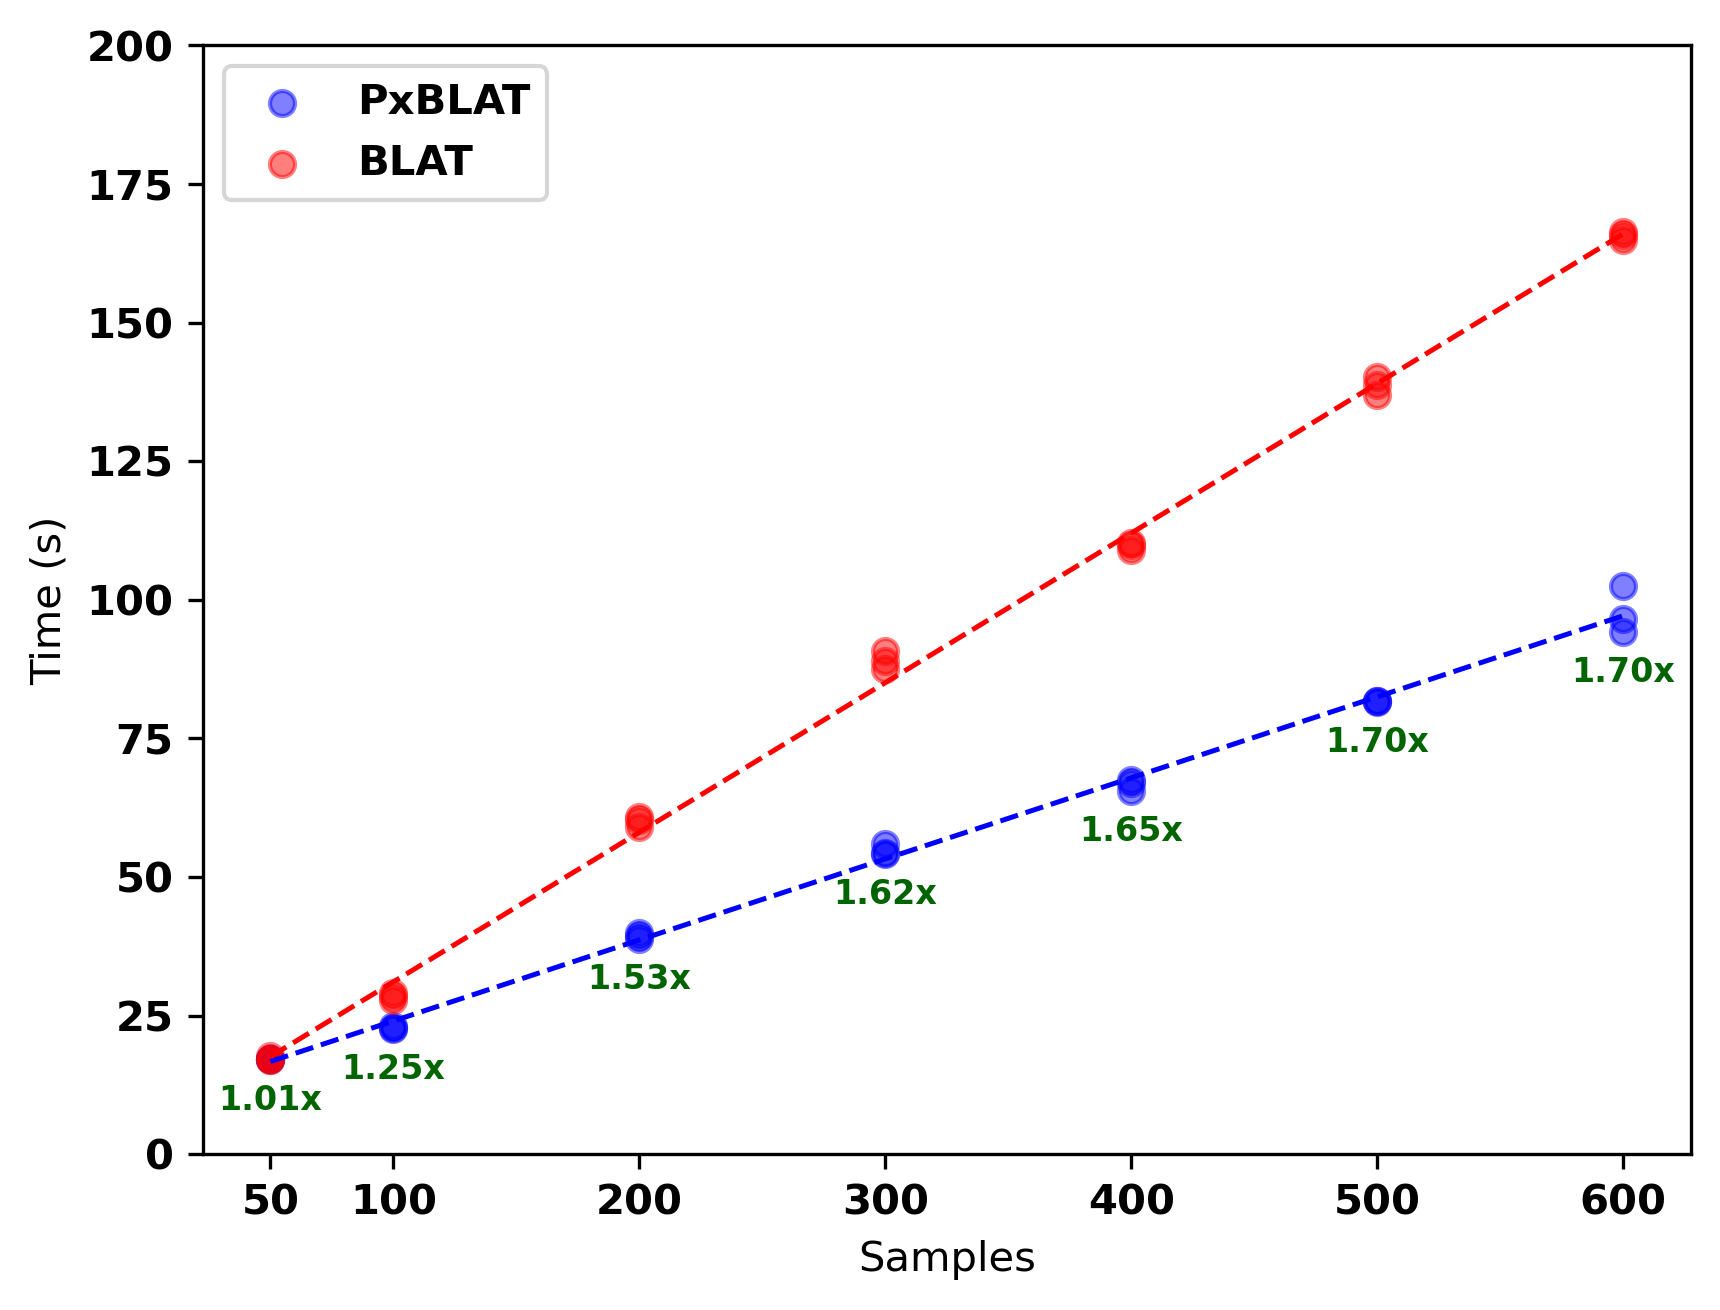
\includegraphics[width=\linewidth]{Fig/performance}
	\caption{Performance Between BLAT and PxBLAT}
	\label{fig:performance}
\end{figure}

The benchmarking was conducted on an Apple M1 Pro with macOS 13.4.1 22F82 arm64.
We use system calls to launch \gls{blat} and the \emph{time} library to measure the execution time.
\gls{pxblat}, on average, gains \SI[per-mode=symbol, round-precision=0]{20}{\percent} speedup compared to \gls{blat}~\pCref{tab:performance-evaluation}.s
In summary, \gls{pxblat}  offers tangible benefits according to reduced execution time and improved user experience, proving its value as an enhancement to \gls{blat}'s functionality.

\section{Acknowledgments}

Special thanks to the team who maintain the \gls{ucsc} codebase and users from the bioinformatics community whose valuable feedback and suggestions were pivotal in refining \gls{pxblat}'s design and functionality.

\section{Competing interests}
No competing interest is declared.

\section{Funding}\label{sec:funding}

This work was supported by the National Institute of General Medical
Sciences [R35GM142441].

\section*{Data availability}\label{sec:data-availability}

The \gls{pxblat}, along with the source code, is publicly available in the GitHub repository at \url{https://github.com/ylab-hi/pxblat}.
The documentation is available at ReadtheDocs \url{https://pxblat.readthedocs.io/en/latest/}.
The script for benchmarking is available at \emph{tests/test\_result.py} in the repository.
The testing dataset is available at the GitHub repository {\url{https://github.com/ylab-hi/pxblat}.
The path of the testing dataset is \emph{benchmark/fas}.

%\bibliographystyle{plain}
%\bibliography{reference}

%USE THE BELOW OPTIONS IN CASE YOU NEED AUTHOR YEAR FORMAT.
\bibliographystyle{abbrvnat}
\bibliography{ref}

%% sample for biography with author's image
% \begin{biography}{{\color{black!20}\rule{77pt}{77pt}}}{\author{Author Name.} This is sample author biography text. The values provided in the optional argument are meant for sample purposes. There is no need to include the width and height of an image in the optional argument for live articles. This is sample author biography text this is sample author biography text this is sample author biography text this is sample author biography text this is sample author biography text this is sample author biography text this is sample author biography text this is sample author biography text.}
% \end{biography}

%% sample for biography without author's image
% \begin{biography}{}{\author{Author Name.} This is sample author biography text this is sample author biography text this is sample author biography text this is sample author biography text this is sample author biography text this is sample author biography text this is sample author biography text this is sample author biography text.}
% \end{biography}

\end{document}
